\section{Implementierung}
\label{implementierung}

Der Fokus der Implementierung liegt darauf, eine Ausreichende Infrastruktur zu schaffen, damit die Implementierung einzelner Erweiterungen keine neuen Herausforderungen aufweist, sofern sie zur Installation keine Schritte erfordern, die in der Konzeptionierung nicht berücksichtigt wurden. Die Implementierung einzelner Erweiterungen geschieht also nur exemplarisch um die Funktionalität des Grundgerüsts und des Ansatzes zu demonstrieren.

\subsection{Umsetzung von Erweiterungen im Allgemeinen}
Bei der Definition von und dem Umgang mit Erweiterungen sind einige allgemeine Probleme erschienen, die unabhängig von der konkreten Erweiterung waren. In diesem Unterkapitel wird auf diese Probleme eingegangen und es wird jeweils erläutert, wie sie gelöst werden konnten.

\subsubsection{Probleme mit zyklischen Codeverweisen}
Aus der Konzeptionierung geht hervor, dass es notwendig ist, dass Erweiterungen gegenseitig aufeinander verweisen können, beispielsweise im Rahmen der Definition von Abhängigkeiten oder Exklusivitäten. Außerdem wurde dargestellt, dass Exklusivitäten symmetrisch sind, d.h. dass $A$ zu $B$ genau dann exklusiv ist, wenn auch $B$ zu $A$ exklusiv ist.

Bei der Implementierung von Erweiterungen wurden die Exklusivitäten daher zunächst auch symmetrisch eingetragen. Dies führte jedoch zu dem Problem, dass die Definitionen dieser Erweiterungen zyklisch aufeinander verwiesen haben. Die Definition der Erweiterung $A$ brauchte eine Referenz auf die Erweiterung $B$, aber $B$ konnte nicht ohne eine Referenz auf $A$ erstellt werden.

In JavaScript wird dieses Problem ohne Ausgabe einer Warnung dadurch gelöst, dass eine von beiden Referenzen den Wert \verb|undefined| annimmt, also dass eine von beiden Erweiterungen eine Exklusivität zu \verb|undefined| erhält.

Dasselbe Problem entsteht auch in anderen, gelegentlich notwendigen Situationen. Wenn beispielsweise ein Framework von einer Erweiterung abhängt (weil sie nicht-optional mit installiert wird, wie z.B. Angular nicht ohne TypeScript installiert werden kann) und dann die Deaktivierungsprüfung dieser Erweiterung beinhaltet, dass geprüft werden muss, ob das Framework ausgewählt wurde, erhält man wieder zyklische Verweise innerhalb der Definitionen der Erweiterungen.

Ein Lösungsansatz für dieses Problem wäre, die Definition und die \glqq Füllung\grqq\ der Erweiterungen getrennt voneinander durchzuführen. So könnte erst für jede Erweiterung ein leeres Objekt definiert werden, auf das frei verwiesen werden könnte. Daraufhin würden diese Objekte erst mit den eigentlichen Inhalten der Erweiterung gefüllt.

Dieser Ansatz führt jedoch zu Konflikten mit TypeScript. Da dieselben Variablen verwendet werden sollen, um zunächst leere und dann gefüllte Objekte zu speichern, müssten diese Variablen entweder sehr allgemeine Typdefinitionen haben, die während der weiteren Implementierung zu größeren Aufwänden führen würde, oder sie müssten zu einem Zeitpunkt falsche Typdefinitionen besitzen. Auch dieser Ansatz ist suboptimal, da an entsprechenden Stellen Fehlermeldungen von TypeScript absichtlich deaktiviert oder umgangen werden müssten.

Stattdessen ist für jedes einzelne Problem, das zu einem zyklischen Codeverweis geführt hat, eine eigene Lösung gefunden worden. Die Identifikation von Erweiterungen wurde anhand des Namens der Erweiterung gewährleistet. Dazu muss sichergestellt sein, dass alle Namen einzigartig sind. Da Abhängigkeiten sowieso nicht zyklisch sein dürfen, ergibt sich hier kein Problem. Bei Exklusivitäten wurde auf die symmetrische Spiegelung verzichtet und so konnte durch geschickte Deklaration von Exklusivitäten jeder dadurch bedingte zyklische Codeverweis eliminiert werden.

Dieser Ansatz könnte noch dadurch erweitert werden, dass die Exklusivitäten an separater Stelle (nach der initialen Definition aller Erweiterungen) definiert werden. Da Exklusivitäten ohnehin optional sind (bei der Konzeptionierung wurde festgelegt, dass eine Erweiterung keine Exklusivitäten haben muss), würde dies sich nicht weiter auf die Typdefinition von Erweiterungen auswirken. Außerdem ist auch eine nachträgliche Herstellung der Symmetrie möglich, wenn sie für einen Algorithmus zwingend notwendig ist.

Da durch die nun umgesetzte Lösung das Problem der undefinierten Abhängigkeiten / Exklusivitäten nicht komplett ausgeschlossen werden konnte und zusätzlich noch notwendig geworden ist, dass die Namen von Erweiterungen stets einzigartig sind, wurden Überprüfungen eingeführt, die die Sinnhaftigkeit der definierten Erweiterungen sicherstellen sollen. Konkret wird hier sichergestellt, dass in keiner Liste von Abhängigkeiten oder Exklusivitäten der Wert \verb|undefined| vorkommt und dass alle Erweiterungen einzigartige Namen besitzen.

Diese Sinnhaftigkeitsüberprüfung ließe sich leicht in die normale Ausführung des \gls{CLI}s einbinden, sodass vor jeder Ausführung gewährleistet ist, dass die Erweiterungen sinnvoll definiert sind. Da sich die Erweiterungen aber nach dem Kompilierprozess nicht mehr verändern, würde es auch ausreichen, die Überprüfungen bei der Gelegenheit auszuführen. Dadurch würde bei Nutzenden etwas Rechenleistung gespart werden.

Eine weitere Möglichkeit ist die Ausführung der Überprüfungen im Rahmen der automatisierten Tests. Diese Variante hat den Nachteil, dass es möglich wäre, eine fehlerhafte Version von \gls{GWA} zu veröffentlichen. Da die Ausführung der Tests im Rahmen dieser Arbeit aber bereits nach jeder Änderung automatisch geschieht und sie für zukünftige Fremdbeiträge ebenfalls über GitHub Actions\footnote{\url{https://github.com/features/actions}} automatisiert werden kann, ist dieses Risiko als vernachlässigbar einzustufen.

Da die Einbindung der Überprüfungen in die automatisierten Tests erheblich einfacher ist als die Einbindung in den Kompilierprozess und die Differenz des bleibenden Risikos nicht bedeutend ist, wurde die Einbindung in die automatisierten Tests vorgenommen.

\subsubsection{Prüfung, ob eine Erweiterung ausgewählt worden ist}
Für verschiedene Features ist es notwendig, dass Erweiterungen feststellen können, ob andere Erweiterungen ebenfalls ausgewählt worden sind (z.B. damit ESLint seine Installation aussetzen kann, falls React ausgewählt wurde, da React bereits ESLint installiert). Diese Feststellung wird unter anderem im Rahmen von Schleifen aufgerufen und sollte daher eine möglichst geringe Laufzeit besitzen.

Ideal wäre daher eine Laufzeit in $\mathcal{O}(1)$. Diese könnte beispielsweise erreicht werden, indem eine Hashmap verwendet wird, sofern die zugehörige Hashfunktion in $\mathcal{O}(1)$ läuft. In dieser Hashmap würde dann er für jede Erweiterung als bool'scher Wert gespeichert werden, ob die Erweiterung ausgewählt wurde.

Da aber beim Start des Programmes alle möglichen Erweiterungen bekannt sind, können diesen eindeutige IDs zugewiesen werden, die dann als Index eines Arrays gelten können, in dem Daten zu den Erweiterungen gespeichert werden. Da die ID jeder Erweiterung bekannt ist, kann so trivialerweise in $\mathcal{O}(1)$ festgelegt und überprüft werden, ob die Erweiterung ausgewählt wurde.

\subsubsection{Überprüfung der Umsetzbarkeit der Restriktionen}
Während  der Implementierung verschiedener Erweiterungen ist es versehentlich passiert, dass eine Konstellation von Restriktionen definiert wurde, die einen inneren Widerspruch enthält.

Da zu erwarten ist, dass verschiedene Leute ohne Kenntnis aller anderen Erweiterungen neue Erweiterungen erschaffen oder bestehende Erweiterungen modifizieren werden, sollte verhindert werden, dass versehentlich solche Kombinationen von Restriktionen erzeugt werden. Daher gilt es, mindestens zu jeder Kompilierzeit alle Restriktionen auf ihre Umsetzbarkeit zu überprüfen und im Falle eines Widerspruchs eine Warnung auszugeben. Da im verwendeten Projektumfeld die Ausführung während der Komiplierzeit sich als etwas schwieriger gestaltet hätte und die Überprüfung dieser Restriktionen nicht merklich lange dauert, wurde diese Überprüfung in die Ausführung der automatischen Tests verschoben.

Ein triviales Beispiel einer unmöglichen Kombination von Restriktionen wäre ein Paar von Abhängigkeiten $A$ und $B$, wobei $A$ und $B$ exklusiv zueinander sind und gleichzeitig $A$ von $B$ abhängt. Es können in diesem Beispiel niemals beide Anforderungen gleichzeitig erfüllt werden.

Natürlich lassen sich aber auch kompliziertere Beispiele erzeugen. In Abbildung \ref{fig:impl:dependency_conflict_examples} werden zwei solche Konstellation dargestellt. Bei der einen hängt $A$ von $B$ und $B$ von $C$ ab, aber $A$ ist zu $C$ exklusiv. Diese Kombination von Anforderungen lässt sich ebensowenig wie das erste Beispiel gleichzeitig erfüllen, aber das Problem ist hier nicht sofort offensichtlich. Man muss hierfür erkennen, dass Abhängigkeiten transitiv sind. Ist also die Erweiterung $A$ von $B$ und $B$ von $C$ abhängig, so ist auch indirekt $A$ von $C$ abhängig.

  \begin{figure}
		\centering
		\begin{subfigure}[a]{0.4\linewidth}
			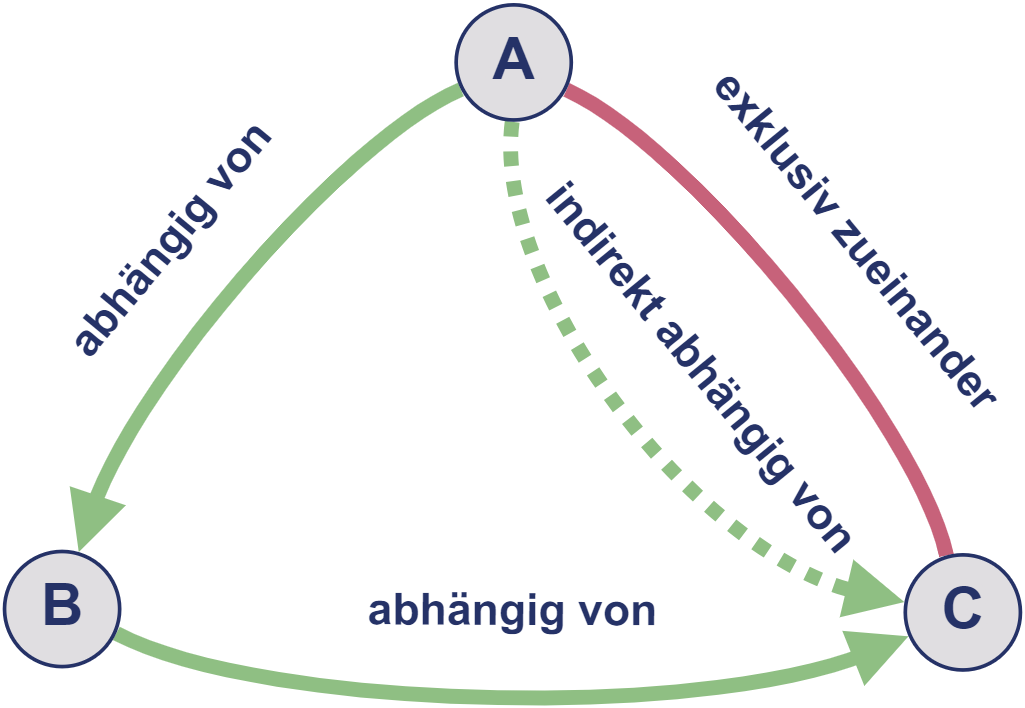
\includegraphics[width=\linewidth]{dependency_example_1.png}
      		\caption{Eine Möglichkeit, wie ein Widerspruch zwischen indirekter Abhängigkeit und Exklusivität entstehen kann.}
		\end{subfigure}
		\begin{subfigure}[a]{0.4\linewidth}
			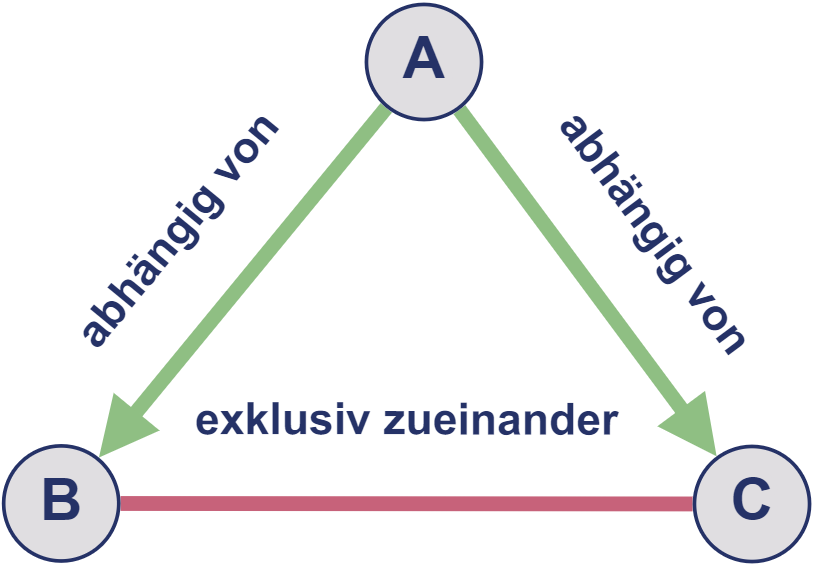
\includegraphics[width=\linewidth]{dependency_example_2.png}
      		\caption{Hier entsteht ein Widerspruch dadurch, dass eine Erweiterung zwei Abhängigkeiten hat, die zueinander exklusiv sind.}
		\end{subfigure}
		\caption{Zwei Graphen zur Veranschaulichung von Konfliktmöglichkeiten zwischen Abhängigkeiten und Exklusivitäten.}
		\label{fig:impl:dependency_conflict_examples}
  \end{figure}

Der zweite in Abbildung \ref{fig:impl:dependency_conflict_examples} dargestellte Konflikt beruht im Gegensatz zu den bisherigen Beispielen nicht darauf, dass eine Erweiterung zugleich (indirekt) abhängig von und exklusiv zu einer anderen Erweiterung ist. Hier wird eine weitere Kategorie von Problemen dargestellt: sind zwei (indirekte) Abhängigkeiten einer Erweiterung zueinander exklusiv, so können nicht beide dieser Abhängigkeiten erfüllt werden. Auch solche Konfigurationen sind also unzulässig.

Aus diesen fachlichen Überlegungen heraus ergibt sich eine erste Lösung. Für jede Erweiterung $E$ sind zunächst alle direkten sowie indirekten Abhängigkeiten zu bestimmen. Für alle diese Abhängigkeiten ist dann zu prüfen, dass zum einen die Abhängigkeit $A$ nicht zu $E$ exklusiv ist, aber auch dass $A$ zu keiner weiteren (indirekten) Abhängigkeit $A'$ von $E$ exklusiv ist.

Bei näherer Betrachtung dieser Lösung lässt sich jedoch einiges an Ineffizienz feststellen. Zum einen werden für jede Erweiterung erneut die transitiven Abhängigkeiten berechnet. Aufgrund eben dieser Transitivität sind jedoch die Berechnungen für alle Erweitungen, die Abhängigkeit einer anderen Erweiterung sind, redundant. Im schlimmsten Fall (nämlich, wenn eine Erweiterung von insgesamt $n$ Erweiterungen von allen anderen Erweiterungen (indirekt) abhängt) ist also genau eine der durchgeführten Berechnungen wirklich notwendig und $n - 1$ Berechnungen werden unnötigerweise durchgefüht. Aus ähnlichem Grund ist auch die Überprüfung der Exklusitivät zweier paarweise unabhängiger (indirekter) Abhängigkeiten häufig überflüssig.

Die Lösung dieser Probleme ergibt sich aus einer theoretischeren Betrachtung des Problems. Wie bereits aus der Verwendung des Begriffs der Transitivität hervorgeht, lassen sich Abhängigkeit und Exklusitivät als mathematische Relationen über der Menge aller Erweiterungen auffassen. Hierbei ist besonders hervorzuheben, dass die Exklusivität symmetrisch ist (ist $A$ zu $B$ exklusiv, so ist auch $B$ zu $A$ exklusiv) während Abhängigkeit nicht symmetrisch ist (im Gegenteil: bei der anfänglichen Analyse von möglichen Bibliotheken, Frameworks etc. ergab sich, dass Abhängigkeit nie symmetrisch zu sein scheint). Allerdings ist Exklusivität a priori nicht transitiv (auch, wenn $A$ zu $B$ und $B$ zu $C$ exklusiv ist, können $A$ und $C$ zusammen verwendet werden), während Abhängigkeit sehr wohl transitiv ist (wie bereits erläutert).

Vor diesem Hintergrund lässt sich erkennen, dass die Bestimmung der (indirekten) Abhängigkeiten der Bestimmung der Transitiven Hülle gleichkommt. Diese kann mittels des Floyd-Warshall-Algorithmus (in der Warshall-Variante) berechnet werden \cite{warshal1_algorithm}. Hierfür muss zunächst ein gerichteter Graph erzeugt werden, in den alle deklarierten Abhängigkeiten als Kante eingefügt werden. Von diesem Graphen wird dann die transitive Hülle bestimmt, in der zwei Knoten $A$ und $B$ genau dann durch eine (von $A$ nach $B$ gerichtete) Kante verbunden sind, wenn die Erweiterung $A$ von $B$ abhängt.

Auch die Relation der Exklusivität lässt sich in einen Graphen überführen. In diesem Graphen gibt es ebenfalls pro Erweiterung einen Knoten und jede Exklusivität wird als Kante dargestellt. Aufgrund der Symmetrie der Exklusivität kann dieser Graph aber ungerichtet sein.

Das Problem der Überprüfung der Restriktionen reduziert sich nun darauf, sicherzustellen, dass es zwischen zwei Knoten (also zwischen zwei Erweiterungen) in maximal einem der beiden Graphen eine Kante gibt, wobei die Richtung keine Rolle spielt (denn wenn die Knoten exklusiv zueinander sind, darf es zwischen beiden keine Abhängigkeit geben -- egal, in welche Richtung).

Anders formuliert, darf es im Graphen der Exklusivitäten keine Kante $\{A, B\}$ geben, für die in der transitiven Hülle der Abhängigkeiten die Kante $(A, B)$ oder die Kante $(B, A)$ existiert. Aufgrund dessen, dass die transitive Hülle gerichtet ist, gibt es darin doppelt so viele Kanten wie in dem Graphen der Exklusivitäten. Außerdem liegt sie als Adjazenzmatrix vor, während die Exklusivitäten als Kantenliste vorliegen. Somit kann bei $m$ Exklusivitäten in $\mathcal{O}(m)$ über die Exklusivitäten iterieren und jeweils in $\mathcal{O}(1)$ die Existenz einer (transitiven) Abhängigkeit prüfen. Die Umkehrung, also die Iteration über Abhängigkeiten und dann die Prüfung der Existenz einer Exklusivität, würde bei $n$ Erweiterungen einen Aufwand von $\mathcal{O}(n^2)$ verursachen. Wenn man vorher die Kantenliste der Exklusivitäten in $\mathcal{O}(n^2)$ in eine Adjazenzmatrix überführt, ist die anschließende Existenzprüfung auch wieder in $\mathcal{O}(1)$ möglich, aber insgesamt

Der Algorithmus von Floyd-Warshall sorgt dafür, dass diese Überprüfung eine asymptotische Laufzeit von $\mathcal{O}(n^3)$ hat. Da die oben beschriebenen Probleme in beliebiger Tiefe von Abhängigkeiten auftreten können, ist jedoch die Bestimmung der transitiven Hülle nicht vermeidbar. Allerdings ist damit zu rechnen, dass die Anzahl aller Erweiterungen stets kleiner als $100$ sein wird (andernfalls würde die Benutzbarkeit des Programms möglicherweise stark eingeschränkt). Daher ist diese Laufzeit in diesem Fall als unbedenklich einzustufen.

Da auch diese Überprüfung sich lediglich auf die Definitionen der Erweiterungen verlässt, wird auch sie in die Ausführung der automatisierten Tests eingebunden, damit sichergestellt werden kann, dass keine fehlerhaften Erweiterungsdefinitionen veröffentlicht werden.

\subsubsection{Überprüfung der getroffenen Auswahl von Erweiterungen}
\label{impl:verify_chosen_extensions}
Um die getroffene Auswahl an Erweiterungen auf die Einhaltung aller Restriktionen hin zu überprüfen, wurde ebenfalls zunächst eine fachliche Lösung gefunden. Für jede der ausgewählten Erweiterungen sind alle Abhängigkeiten und Exklusivitäten durchzugehen. Ist eine Abhängigkeit nicht mit ausgewählt worden oder ist eine Exklusivität mit ausgewählt worden, so ist (genau dann) die Kombination ungültig.

Die Laufzeit dieses Vorgehens liegt für $n$ mögliche Erweiterungen in $\mathcal{O}(n^3)$ (mit Möglichkeit der Reduktion auf $\mathcal{O}(n^2)$). Dies liegt daran, dass zunächst über jede der (maximal $n$) ausgewählten Erweiterungen und dann über jede der Abhängigkeiten und Exklusivitäten iteriert werden muss. Da eine Erweiterung niemals zu einer Abhängigkeit exklusiv sein kann, beträgt die Summe der Abhängigkeiten und Exklusivitäten maximal $n$. Somit ist bereits eine Laufzeit von $\mathcal{O}(n^2)$ erreicht worden.

Nun bleibt noch die Prüfung, ob eine Abhängigkeit bzw. Exklusivität ausgewählt worden ist oder nicht, d.h. ob sie in der Liste der ausgewählten Erweiterungen liegt oder nicht. Im Falle einer normalen Liste läge die Laufzeit dieser Überprüfung bei $\mathcal{O}(n)$, da die im schlimmsten Fall die gesamte Liste überprüft werden müsste. Allerdings kann man diese Information auch als Liste bool'scher Werte speichern, wobei unter jedem Index genau eingetragen ist, ob die Erweiterung mit demselben Index in der Liste aller möglichen Erweiterungen ausgewählt worden ist. So wäre die Überprüfung der Auswahl einer einzelnen Erweiterung in $\mathcal{O}(1)$ möglich und würde die Gesamtlaufzeit nicht weiter beeinflussen.

Ähnlich wie bei der Überprüfung der Umsetzbarkeit aller Restriktionen lässt sich jedoch auch für dieses Problem eine graphentheoretische Lösung finden. Da bereits Graphen bestimmt wurden, in denen Kanten für Abhängigkeit und Exklusivität eingetragen sind, können diese zunächst kopiert und dann zur Überprüfung dieses Problems verwendet werden. Die Kopie erfolgt in $\mathcal{O}(n^2)$, da eine $n \times n$-Adjazenzatrix und eine Kantenliste mit maximal Länge $n^2$ kopiert werden müssen.

Im Graphen der Abhängigkeiten sind Kanten nun als noch unerfüllte Bedingungen anzusehen. Die Streichung einer Kante bedeutet somit, dass die entsprechende Bedingung erfüllt ist. Nun ist über jede mögliche Erweiterung zu iterieren. Falls sie ausgewählt worden ist, so sind auf sie eingehende Kanten aus dem Graphen der Abhängigkeiten zu streichen. Andernfalls (d.h. wenn sie nicht ausgewählt worden ist) ist ihr Knoten mitsamt seiner ausgehenden Kanten zu streichen. Es sind genau dann alle Abhängigkeiten erfüllt, wenn nach der Iteration über alle möglichen Erweiterungen keine Kanten mehr in dem Graphen vorhanden sind.

Ähnlich ist für die Exklusivitäten zu verfahren. In diesem Graphen bedeutet die Existenz einer Kante, dass die zugehörige Exklusivität in der aktuellen Auswahl noch nicht ausgeschlossen werden konnte. Während über alle Erweiterungen iteriert wird, kann also für jede nicht ausgewählte Erweiterung der zugehörige Knoten zusammen mit seinen (ungerichteten) Kanten gestrichen werden. Auch die Exklusivitäten sind alle genau dann erfüllt, wenn sich am Ende der Iterationen keine Kante mehr im Graphen befindet.

Der erste Aspekt der Laufzeit dieser Verfahren ergibt sich dadurch, dass die Graphen in verwendbarer und modifizierbarer Form vorliegen müssen (d.h. als neu angelegte Adjazenzmatrizen). Die im letzten Kapitel berechnete Adjazenzmatrix der Abhängigkeit muss also lediglich kopiert werden, während der Graph der Exklusivität in eine Adjazenzmatrix überführt werden muss. Dies kann in $\mathcal{O}(n^2)$ geschehen.

Danach muss über jede Erweiterung iteriert werden und ggf. (also falls sie nicht ausgewählt wurde) die zugehörige Zeile und Spalte der Adjazenzmatrix modifiziert werden. Anschließend muss die gesamte Matrix auf die Existenz von Kanten hin überprüft werden. Beide Schritte geschehen nacheinander in jeweils $\mathcal{O}(n^2)$. Somit fordert der gesamte Prozess eine Laufzeit von $\mathcal{O}(n^2)$.

Alternativ zu den Adjazenzmatrizen könnten auch Kantenlisten verwendet werden. Dann müsste aber für die Löschung von Knoten, die in beiden Prozessen maximal für jede Erweiterung vorkommen könnte, jeweils die gesamte Liste durchlaufen werden. Es entstünde also auch hier ein Aufwand von $\mathcal{O}(n^2)$.

Die Betrachtung der Graphentheoretischen Lösung ergibt also in diesem Fall keine Verbesserung der Laufzeit. Nach persönlichem Empfinden ist die erste Lösung jedoch leichter zu verstehen und wurde angesichts der gleichen Laufzeit aufgrund dieses Kriteriums ausgewählt und umgesetzt.

\subsection{Umsetzung des Dialogs}
Der Dialog mit Nutzenden lässt sich grob in drei Aufgaben unterteilen. Die erste Aufgabe ist das Untersuchen der \gls{CLI}-Argumente. In diesem Schritt werden keine Ausgaben erzeugt, aber da er auf einer manuellen Eingabe operiert, zählt er trotzdem zum Prozess des Dialogs.

Mit den vorgegebenen Optionen werden dann, sofern notwendig, weitere allgemeine Fragen gestellt. Hier haben Nutzende die Möglichkeit, den Namen des Projektes anzugeben, einen Paketmanager und die gewünschten Erweiterungen auszuwählen. Ist eine dieser Fragen bereits in den \gls{CLI}-Argumenten beantwortet worden, so kann die entsprechende Frage übersprungen werden.

Als letzten Schritt des Dialogs sind dann weitere Fragen der einzelnen Erweiterungen zu stellen. Auch diese können bereits beantwortet worden sein und werden ggf. übersprungen.

\subsection{Analyse der CLI-Argumente}
Mithilfe der bereits erwähnten Bibliothek \glqq commander\grqq können die \gls{CLI}-Argumente mit sehr geringem Aufwand eingelesen und in gewissem Rahmen validiert werden. Dazu ist es notwendig, alle möglichen Argumente und ggf. die Typen der erwarteten zugehörigen Werte zu deklarieren.

Für die Angabe eines bool'schen Wertes reicht dann ein Parameter ohne zugehörigen Wert (z.B. \verb|--use-some-library|), während Angabe einer Wahl von bestimmten Optionen zusätzlich die Angabe eines Wertes benötigt (z.B. \verb|--package-manager npm|). Commander erzeugt bei der anschließenden Analyse der beim Befehlsaufruf übergebenen Argumente ein Objekt, bei dem jedem angegebenen Argument der entsprechende Wert (oder, falls kein Wert angegeben wurde, der bool'sche Wert \verb|true|) zugewiesen ist. Wenn eine Option beim Befehlsaufruf nicht angegeben wurde, so wird sie in das ausgegebene Objekt nicht aufgenommen.

Bool'sche Optionen können daher nicht durch Weglassung auf den Wert \verb|false| gesetzt werden. Um sie trotzdem negierbar zu machen, kann man eine weitere Option mit dem Präfix \verb|no-| erstellen (z.B. \verb|--no-use-some-library|). Diese wird von commander automatisch als Negation der zugehörigen Option (in dem Beispiel also der Option \verb|--use-some-library|) erkannt. Natürlich kann dieselbe Funktionalität auch mit anderen Benamungen umgesetzt werden; dies ist dann aber mit höherem Aufwand verbunden, da die zugehörige Logik von Hand implementiert werden muss.

Um alle Fragen, die im Laufe des Dialogs gestellt werden könnten, durch solche \gls{CLI}-Argumente abzudecken, muss es möglich sein, dass Erweiterungen ebenfalls Argumente deklarieren können. Dies wird umgesetzt, indem Erweiterungen eine Funktion definieren können, die auf dem überreichten commander-Objekt frei Argumente definieren kann.

Daraufhin werden die Argumente von commander analysiert. Die allgemeinen Metadaten werden herausgefiltert und an die Stellung der entsprechenden Fragen weitergegeben. Alle weiteren Argumente können im allgemeinen Teil jedoch nicht weiter verarbeitet werden und müssen daher als Gesamtheit im Rahmen des weiteren Dialogs an die Erweiterungen überreicht werden (siehe Abschnitt \ref{impl:extension_questions}).

Vor der Weitergabe der per \gls{CLI}-Argumente übergebenen allgemeinen Daten müssen diese jedoch validiert werden. Insbesondere bezieht sich dies auf die Überprüfung der Auswahl der Erweiterungen (siehe Kapitel \ref{impl:verify_chosen_extensions}). Sofern keine Erweiterung per \gls{CLI}-Argument ausgewählt wurde, kann diese Validierung übersprungen werden, da die zugehörige Frage später gestellt werden muss und die Validierung dabei erfolgen kann.

Weniger eindeutig ist jedoch, wie mit der Angabe einer oder mehrerer gewünschter Erweiterung(en) per \gls{CLI}-Argumente umzugehen ist, da nicht eindeutig erkennbar ist, ob die so getroffene Auswahl vollständig sein soll. Falls sie nicht vollständig wäre, müsste die zugehörige Frage gestellt werden, was aber eine programmatische Verwendung von \gls{GWA} deutlich erschweren würde. Daher ist davon auszugehen, dass die per \gls{CLI}-Argumente getroffene Auswahl an Erweiterungen vollständig ist, sobald mindestens eine Erweiterung ausgewählt wurde. In diesem Fall ist dann die Überprüfung dieser Auswahl durchzuführen und im Fehlerfall ist die Ausführung von \gls{GWA} abzubrechen.

\subsubsection{Stellen allgemeiner Fragen}
\label{impl:general_questions}
In diesem Abschnitt des Dialogs werden sowohl Metadaten des zu erzeugenden Projektes gesammelt als auch die Auswahl der zu installierenden Erweiterungen getroffen. Die Sammlung der Metadaten ist ohne besonderen Aufwand umsetzbar, da alle hierfür relevanten Fragetypen (Freitext-Eingabe, Auswahl eines von $n$ Elementen) von inquirer zur Verfügung gestellt werden und direkt verwendet werden können.

Bemerkenswert ist lediglich, dass vor der Frage, welcher Paketmanager verwendet werden soll, geprüft wird, welche Paketmanager überhaupt installiert sind. Auch, wenn nur ein Paketmanager installiert ist und somit gar keine Auswahl getroffen werden kann, wird die Frage gestellt und erhält lediglich ergänzende Bemerkungen, dass andere Paketmanager nicht zur Verfügung stehen. Diese Entscheidung wurde getroffen, um unerfahrene Entwickelnde zumindest darüber zu informieren, dass es weitere Paketmanager gibt. Außerdem kann diese Frage leicht übersprungen werden, indem die entsprechende Entscheidung per \gls{CLI}-Argument \verb|--package-manager| spezifiziert wird. Um dies weiter zu erleichtern, wurde auch der Alias \verb|-p| eingerichtet.

Die Frage zur Auswahl der zu installierenden Erweiterungen gestaltet sich etwas schwieriger. Sie muss von einer allgemeinen Stelle aus gestellt werden, da sie erweiterungsübergreifend ist, aber muss dennoch erweiterungsspezifische Inhalte darstellen können. Um auch diese Frage möglichst verständlich und informativ zu gestalten, müssen Erweiterungen neben ihrem Namen auch eine Kurzbeschreibung, einen Link zu mehr Informationen und die Kategorie der Erweiterung angeben. Name, Kurzbeschreibung und Link werden in die Frage eingebaut, während die Kategorie lediglich für eine sinnvolle Gruppierung und Trennung der Erweiterungen genutzt wird.

Inquirer ermöglicht bei allen Fragen die Angabe einer Funktion, die eine Antwort auf die Frage entgegennimmt und diese validiert. Auf diesem Weg ist es möglich, die in Kapitel \ref{impl:verify_chosen_extensions} beschriebene Überprüfung der getroffenen Auswahl durchzuführen. Wird ein Fehler festgestellt, so wird dieser von inquirer ausgegeben und die Frage wird beibehalten, bis eine Antwort die Validierung besteht. So wird garantiert, dass die weiteren Schritte von \gls{GWA} nicht ausgeführt werden können, bis eine gültige Auswahl von Erweiterungen getroffen wurde.

\subsubsection{Übergabe des Dialogs an Erweiterungen}
\label{impl:extension_questions}

Da auch Erweiterungen in der Lage sein müssen, im Rahmen des Dialogs Fragen zu stellen, können sie eine Funktion definieren, die nach dem Stellen eventueller Fragen ein Objekt zurück gibt, das die aus den Fragen resultierende Konfiguration enthält. Damit keine bereits beantworteten Fragen gestellt werden und die per \gls{CLI}-Argumente spezifizierten Optionen bei der Erzeugung dieses Konfigurationsobjektes berücksichtigt werden können, müssen alle \gls{CLI}-Argumente ebenfalls an diese Funktion übergeben werden.

Um den Dialog möglichst übersichtlich zu gestalten, ist es sinnvoll, die Fragen einzelner Erweiterungen visuell voneinander zu trennen, damit Nutzenden bewusst ist, worauf sich jede aktuelle Frage bezieht. Hierfür soll vor den Fragen jeder Erweiterung der Name der Erweiterung als Überschrift der folgenden Fragen ausgegeben werden. Außerdem soll zwischen den Fragen der letzten Erweiterung und der Überschrift der Fragen der nächsten Erweiterung eine Leerzeile eingefügt werden.

Um diese Formatierung zu garantieren und möglichst wiederholungsfreien Code zu erzeugen, ist diese Formatierung außerhalb der Erweiterungen umzusetzen. Dies hat zudem den Vorteil, dass Randfälle (z.B. Ausgaben vor der ersten / nach der letzten Erweiterung) leichter betrachtet werden können, da Erweiterungen beim Stellen von Fragen nicht wissen, ob vor oder Nach ihnen Fragen gestellt wurden / werden.

Diese Umsetzung ist jedoch fehlerhaft, falls aufgrund von \gls{CLI}-Argumenten bestimmte Fragen ausgesetzt werden. Wenn alle Fragen einer Erweiterung ausgesetzt werden, dann sollte für die Erweiterung auch keine Leerzeile oder Überschrift ausgegeben werden, was bei dem bisher beschriebenen Ansatz aber geschehen würde.

Um dieses Problem zu lösen, wird an die Funktionen zum Stellen von Fragen als weiterer Parameter eine Funktion übergeben, die zunächst nur inquirer ummantelt und jeden Aufruf direkt weiterleitet. Vor der Weiterleitung eines Aufrufes prüft sie jedoch, wie viele Fragen gestellt werden. Sobald eine Erweiterung (mindestens) eine Frage stellt, gibt sie vor dem Weiterleiten die trennende Leerzeile sowie die Überschrift aus. Stellt eine Erweiterung also keine Fragen, wird beides nicht ausgegeben.

Dieses Vorgehen hat auch den Vorteil, dass mit besonders geringem Aufwand im Rahmen der automatischen Tests das Stellen von Fragen gesteuert werden kann, ohne, dass die Ausgaben der Tests von Ausgaben von inquirer unterbrochen werden. Hierfür muss lediglich die übergebene Funktion darauf verzichten, inquirer aufzurufen und im Rahmen der Tests gewünschte Antworten ohne das Stellen entsprechender Fragen zurück geben.

\subsection{Installation von Erweiterungen}
Nachdem alle benötigten Informationen eingeholt und verifiziert worden sind, ist nun die Installation der Erweiterungen durchzuführen. Hierfür wird in einer bestimmten Reihenfolge (siehe Kapitel \ref{impl:determine_installation_order}) für jede der ausgewählten Erweiterungen zunächst geprüft, ob sie übersprungen werden soll. Falls dem nicht so ist, wird dann eine von ihr definierte Funktion zur Installation aufgerufen. Diese erhält als Parameter alle gesammelten Metadaten sowie die zum gewählten Paketmanager gehörige Strategie und eine Liste mit allen ausgewählten Erweiterungen mitsamt ihren speziell getroffenen Einstellungen.

Um Nutzenden den Fortschritt von \gls{GWA} mitzuteilen, wird vor dem Aufruf der Installationsfunktion ausgegeben, dass nun mit der Installation der entsprechenden Erweiterung begonnen wird. Diese Meldung wird nicht ausgegeben, wenn die Erweiterung übersprungen wird. Dies ist der Grund, warum das Überspringen der Installation einer Erweiterung gesondert überprüft werden muss, anstatt ggf. in der Installationsfunktion nichts auszuführen.

Im Anschluss an alle Installationen haben Erweiterungen die Möglichkeit durch eine von ihnen definierte Funktion weitere Informationen auszugeben. Dies kann beispielsweise genutzt werden, um erste Schritte mit einem Framework zu erläutern oder erneut auf die Dokumentation zu verweisen.

\subsubsection{Bestimmung der Installationsreihenfolge}
\label{impl:determine_installation_order}
Wie bereits in der Konzeptionierung erläutert wurde, muss es möglich sein, die Installationsreihenfolge der Erweiterungen festzulegen. Dabei ist nicht die Festlegbarkeit der gesamten Reihenfolge relevant, sondern es müssen lediglich gewisse Bedingungen eingehalten werden.

Beispielsweise muss das Framework zuerst installiert werden, da es die notwendige Ordnerstruktur erzeugt. Die Installation von husky und ESLint sollte sehr spät erfolgen, damit alle im Projekt existierenden Dateiendungen bei entsprechenden Skripten berücksichtigt werden können. Dies sind also zwei Beispiele für \glqq globale\grqq Bedingungen die von einer Erweiterung an den gesamten Kontext gestellt werden.

Es gibt aber auch eine weitere Art von Bedingung, bei der eine Erweiterung nicht vor einer anderen Erweiterung installiert werden darf. Ein solches Beispiel ist, dass husky nach Prettier und ESLint installiert werden muss, da sonst bei den durch husky eingerichteten Automatisierungen die anderen Werkzeuge nicht einbezogen werden. Dieses Konzept ähnelt dem der Abhängigkeiten, kann jedoch ausdrücklich nicht durch die bereits existierenden Abhängigkeiten zwischen Erweiterungen abgebildet werden. Sonst müsste beispielsweise TypeScript vor Angular installiert werden, da Angular von TypeScript abhängig ist. Dies ist jedoch nicht möglich, da (wie bereits erläutert) Frameworks als allererstes installiert werden müssen.

Obwohl sich diese Anforderungen wie geschehen kategorisieren lassen, stellen sie eher eine Ansammlung von Einzelfällen dar. Neben Frameworks gibt es keine Erweiterungen, die als erstes oder letztes zu installieren sind. Die Anforderung von Husky und ESLint ist nach bisherigem Kenntnisstand ebenfalls ein Einzelfall. Da nur begrenzt viele Bibliotheken und Werkzeuge analysiert wurden, kann es darüber hinaus sein, dass es noch weitere Arten von Bedingungen an die Installationsreihenfolge gibt, die für zukünftige Erweiterungen relevant werden. Die einzige Anforderung, die häufig festgestellt wurde, war die, dass eine Erweiterung nicht vor einer oder mehreren anderen installiert werden darf.

Alternativ kann durch händisches Festlegen der Installationsreihenfolge gewährleistet werden, dass sämtliche Anforderungen erfüllt werden. Dieser Ansatz hat den Nachteil, dass er unübersichtlicher ist und leichter bei der Ergänzung neuer Erweiterungen Fehler gemacht werden können. Dafür ist der Implementierungsaufwand deutlich geringer.

Insbesondere, da die Implementierung der bisher beobachteten Anforderungen in Form von inhaltlichen Regeln keine Zukunftssicherheit bietet und dennoch deutlich komplexer wäre, wurde nach der zweiten vorgestellten Methode vorgegangen. Alle Auswählbaren Erweiterungen wurden in einem Array derart aufgelistet, dass die Reihenfolge der Erweiterungen in dem Array die Installationsreihenfolge festlegt. Dieses Array wird zugleich überall dort verwendet, wo eine vollständige Liste aller Erweiterungen benötigt wird.

\subsubsection{Erzeugung von TypeScript- und JavaScript-Dateien}
Im Rahmen der Installation vieler Erweiterungen sind JavaScript- bzw. TypeScript-Dateien (mit entsprechendem Code) zu erzeugen. Hierfür lassen sich trivialerweise Beispieldateien anlegen, von denen dann gemäß der getroffenen Auswahl die richtige ausgewählt und in das neue Projekt kopiert wird. Dieser Ansatz hat jedoch den Nachteil, dass er viel Code verursachen würde, der (bis auf die Existenz von Typen) dupliziert wäre. Das würde die Wartung etwas aufwändiger und unangenehmer machen.

Zudem könnten zwei in diesem Sinne äquivalente Dateien versehentlich verschieden bearbeitet werden, sodass in nur einer der beiden Dateien ein Fehler eingeführt wird. Derartige Fehler können nur durch sehr ausgiebiges Testen gefunden werden und bleiben daher leicht unbemerkt.

Aus diesen Gründen wurde ein Ansatz entwickelt, der aus nur einer Vorlage sowohl entsprechende JavaScript- als auch TypeScript-Dateien erzeugen kann. Mithilfe des TypeScript-Kompilers, der ohnehin aus Entwicklungsgründen in das Projekt eingebunden ist, kann TypeScript-Code zu JavaScript-Code umgewandelt werden. Der Kompiler akzeptiert dabei ein Konfigurationsobjekt, in dem festgelegt werden kann, mit welcher Version des EcmaScript-Standards das JavaScript kompatibel sein soll. Indem hier der neuste Standard spezifiziert wird, ähnelt der resultierende JavaScript-Code maximal dem ursprünglichen Code.

Beim Kompilieren werden jedoch zuvor vorhandene Leerzeilen entfernt, die aus Formatierungs- und Verständlichkeitsgründen relevant sind. Viele dieser Zeichen lassen sich wieder einfügen, indem das Kompilat mit Prettier formatiert wird. Bei einigen Durchläufen dieses Prozesses mit verschiedenen Dateien ist jedoch aufgefallen, dass Leerzeilen, die zur gedanklichen Trennung von Codeblöcken eingefügt wurden, nicht von Prettier wiederhergestellt werden konnten.

Um auch diese Leerzeilen in die generierten JavaScript-Dateien aufnehmen zu können, wird nach dem Kompilieren das Kompilat mit dem ursprünglichen Code verglichen. Dadurch werden entfernte Leerzeichen / -zeilen gefunden und wieder in das Kompilat eingefügt. Hierbei werden jedoch in bestimmten Fällen zu viele Zeichen eingefügt (z.B. werden Leerzeilen, die aufgrund von Typdefinitionen notwendig waren, eingefügt, obwohl die Typdefinitionen nicht mehr vorhanden sind und damit die Leerzeichen / -zeilen nicht benötigt werden). Diese überflüssigen Zeichen können jedoch zuverlässig mit Prettier entfernt werden, solange der ursprüngliche Code den Formatierungsregeln entspricht, mit denen Prettier aufgerufen wird.

Auf diese Art und Weise ist es also möglich, Dateivorlagen in TypeScript zu schreiben und zu pflegen, die bei der Projektinstallation entweder direkt kopiert oder zunächst zu JavaScript umformatiert und dann in das neue Projekt eingefügt werden. Durch die Verwendung des tatsächlichen TypeScript-Kompilers kann garantiert werden, dass die auf diese Art erzeugten Dateien dieselbe Funktionalität bieten.

\subsubsection{Framework-spezifische Codegeneration}
Neben solchem Allgemeinen \gls{JS}- / \gls{TS}-Code muss für einige Erweiterungen auch Framework-spezifischer Code erzeugt werden. Dies ist vor allem dann der Fall, wenn Komponenten oder CSS-Bibliotheken zum Projekt hinzugefügt werden sollen.

Die Anforderungen, die hierfür existieren, sind zwischen den Frameworks teilweise unterschiedlich. In allen Frameworks gibt es jedoch eine Datei, in der die oberste Stufe der \gls{DOM}-Struktur erzeugt wird (in Angular ist dies die \verb|src/app/app.component.html|, in React ist es die \verb|src/App.tsx| und in Vue.js ist es die \verb|src/App.vue|), in die neue Komponenten einzufügen sind.

Dieses Einfügen neuer Komponenten soll immer an derselben Stelle erfolgen, sodass sich dort alle neuen, durch Erweiterungen hinzugefügten Komponenten nacheinander ansammeln. Eine Fachlich orientierte Lösung wäre also in der Lage, den aus den genannten Dateien resultierenden \gls{DOM}-Baum in ein \gls{JS}-Objekt zu überführen, dieses um die gewünschte Komponente zu ergänzen und dann den Objekt entsprechendem Code in die Datei zu schreiben. Die so vorgenommene Änderung sollte minimal und korrekt formatiert sein.

Alternativ dazu wäre es, da diese entsprechenden Dateien bei jeder Installation gleich sind, möglich, über reine Textsuche die Stelle zu finden, in der die neue Komponente einzusetzen ist. Dort würde der entsprechende Code eingefügt werden und anschließend würde mithilfe von Prettier die korrekte Formatierung der Datei gewährleistet werden.

Aufgrund der verschiedenen Syntaxen der drei Frameworks müsste beschriebene fachliche Lösung für jedes Framework einzeln entwickelt werden, was nur mit hohem Aufwand umsetzbar wäre. Der Text-basierte Ansatz wäre sehr fragil, da bereits geringfügige Änderungen der durch Frameworks erzeugten Dateien dazu führen könnten, dass neue Komponenten nicht mehr eingefügt werden können.

Da aber auch der fachliche Ansatz von der genauen \gls{DOM}-Struktur abhängt, die erzeugt werden würde, ist auch er für solche Fehler anfällig. Aufgrund der deutlich geringeren Komplexität wurde deshalb der Text-basierte Ansatz bevorzugt und für alle Frameworks implementiert.

Neben dem Einfügen von Komponenten gibt es noch weitere Änderungen, die vornehmbar sein müssen. In einem Angular-Projekt muss es möglich sein, bestimmte Arrays in einer TypeScript-Datei zu modifizieren. In React-Projekten hingegen muss es möglich sein, neue \gls{DOM}-Elemente derart hinzuzufügen, dass sie andere (bereits existierende) Elemente umgeben. Beide Probleme wurden ebenfalls aus den bereits beschriebenen Gründen mit text-basierten Ansätzen gelöst.

\subsection{Probleme}
Während der Entwicklung sind einige Probleme aufgetreten, mit denen bei der Konzeptionierung nicht gerechnet worden ist. Die folgenden Unterkapitel beschreiben diese Probleme und wie sie gelöst worden sind.

\subsubsection{Falsche Typdefinitionen von inquirer}
Wie bereits beschrieben worden ist, wurde für die Entwicklung von \gls{GWA} TypeScript verwendet. Da aber einige der verwendeten Bibliotheken, darunter inquirer \missingQuote (einfach package.json, Abwesehnheit von typescript), nicht in TypeScript entwickelt wurden und auch keine eigenen von Hand erzeugten Typdefinitionen beinhalten, müssen diese Typdefinitionen aus dritten Quellen bezogen werden.

Dieses Problem ist weit verbreitet und kann häufig mittels des DefinitelyTyped-Projektes gelöst werden \missingQuote (vlt etwas darüber, dass NPM DT-Icon anzeigt). Dies ist ein großes Projekt, was für derartige \gls{npm}-Pakete Typdefinitionen sammelt und als gesonderte \gls{npm}-Pakete veröffentlicht \missingQuote (einfach README).

\begin{lstlisting}[caption={TypeScript-Fehlermeldung bei der Verwendung von inquirer mit einem RxJS-Observable}, captionpos=b, label={code:inquirer_ts_error}]
TS2345: Argument of type
'Observable<DistinctQuestion<Answers>>' is not assignable to
parameter of type 'QuestionCollection<Answers>'.
  Type 'Observable<DistinctQuestion<Answers>>' is missing the
  following properties from type
  'Observable<DistinctQuestion<Answers>>':
  _isScalar, _trySubscribe, _subscribe
\end{lstlisting}

Zu Beginn der Entwicklung ist der in Listing \ref{code:inquirer_ts_error} aufgeführte TypeScript-Fehler entstanden, der sich nicht durch Fehler im selbstgeschriebenen Code erklären lies. Besonders ungewöhnlich an dem Fehler ist, dass zwei identisch benannte Typen (woraus in der Regel folgt, dass die Typen auch tatsächlich identisch sind) zueinander inkompatibel sind.

Bei Nachforschungen in den Abhängigkeiten, aus denen die beiden betroffenen Werte stammten, stellte sich heraus, dass zwei Verschiedene Versionen von RxJS verwendet wurden, deren Typdefinitionen zueinander inkompatibel waren. Konkret hatten die aus DefinitelyTyped stammenden Typdefinitionen von inquirer eine Abhängigkeit auf eine veraltete Version von RxJS deklariert, während \gls{GWA} von der aktuellen Version abhängig war.

Dieser Fehler lässt sich auf zwei Wege lösen. Durch die einfache Löschung der lokalen Installation der veralteten Version von RxJS wird automatisch in den Typdefinitionen von inquirer die (weiterhin installierte) aktuelle Version von RxJS verwendet. Diese Lösung hat allerdings den Nachteil, dass die Löschung der veralteten Version nach jeder Installation oder Verlinkung von \gls{GWA} mit \gls{npm} erneut vorgenommen werden muss, da sie im Rahmen der entsprechenden Befehle erneut installiert wird.

Alternativ kann die Abhängigkeit der Typdefinitionen von inquirer aktualisiert werden. Hierfür wurde in dem DefinitelyTyped-Repository ein Pullrequest gestellt\footnote{\url{https://github.com/DefinitelyTyped/DefinitelyTyped/pull/54885}}, der aber aufgrund mehrerer anderer Abhängigkeiten auf diese Typdefinitionen besondere Überprüfung erforderte.

Während diese Überprüfung stattfand, konnte das Problem mit dem ersten Lösungsansatz umgangen werden. Seit der am 6. September 2021 veröffentlichten Version 8.1.0 der Typdefinitionen von inquirer ist das Problem jedoch gänzlich gelöst.

\subsubsection{Betriebssystemspezifische Probleme}
\subsection{Testgetriebene Entwicklung}